% !TeX program = xelatex
\documentclass[10pt,a4paper]{ctexart} % 设置文章类型，正文字号与纸张大小

% 页面与正文常用宏包
\usepackage[margin=2cm]{geometry} % 设置页面四周页边距
\usepackage{graphicx}             % 插入图片
\usepackage{amsmath}              % 提供cases、aligned等数学公式环境
\usepackage{amssymb}              % 提供\therefore等扩展数学符号
\usepackage{booktabs}             % 提供\toprule、\midrule、\bottomrule三线表命令
\usepackage{float}                % 提供[H]固定图片、表格位置
\usepackage{subcaption}           % 提供subfigure子图环境及子图标题
\usepackage{wrapfig}              % 提供wrapfigure图文环绕环境
\usepackage{fancyhdr}             % 自定义页眉和页脚
\usepackage{hyperref}             % 生成超链接

% 页眉页脚
\pagestyle{fancy}                  % 启用fancyhdr定义的页面样式
\fancyhf{}                         % 清空默认页眉和页脚
\fancyfoot[C]{\thepage}            % 在页脚中央显示页码
\renewcommand{\headrulewidth}{0pt} % 隐藏页眉横线
\renewcommand{\footrulewidth}{0pt} % 隐藏页脚横线

% 超链接
\hypersetup{
  colorlinks=true,                % 使用彩色文字链接，而非带边框的链接
  linkcolor=red,                 % 目录、公式及图表交叉引用的颜色
  filecolor=cyan,                 % 本地文件链接的颜色
  urlcolor=blue,                  % 网址链接的颜色
  pdftitle={光电效应测定普朗克常量预习报告},     % 写入PDF文档属性的标题
  bookmarksnumbered=true          % PDF书签显示章节编号
}

% 定义字号命令
\newcommand{\chuhao}{\fontsize{42pt}{63pt}\selectfont}
\newcommand{\xiaochu}{\fontsize{36pt}{54pt}\selectfont}
\newcommand{\yihao}{\fontsize{26pt}{39pt}\selectfont}
\newcommand{\xiaoyi}{\fontsize{24pt}{36pt}\selectfont}
\newcommand{\erhao}{\fontsize{22pt}{33pt}\selectfont}
\newcommand{\xiaoer}{\fontsize{18pt}{27pt}\selectfont}
\newcommand{\sanhao}{\fontsize{16pt}{24pt}\selectfont}
\newcommand{\xiaosan}{\fontsize{15pt}{22.5pt}\selectfont}
\newcommand{\sihao}{\fontsize{14pt}{21pt}\selectfont}
\newcommand{\xiaosi}{\fontsize{12pt}{18pt}\selectfont}
\newcommand{\wuhao}{\fontsize{10.5pt}{15.75pt}\selectfont}
\newcommand{\xiaowu}{\fontsize{9pt}{13.5pt}\selectfont}

% 章节格式
\ctexset{
  section={
    format={\CJKfontspec[AutoFakeBold=2.5]{KaiTi}\sanhao\bfseries}, % 一级标题使用三号加粗楷体
    name={,、},                                                    % 在中文章节序号后添加顿号
    number=\chinese{section},                                      % 一级标题编号使用“一、二、三”形式
    aftername={}                                                   % 取消编号与标题文字之间的空格
  },
  subsection={
    format={\CJKfontspec[AutoFakeBold=2.5]{KaiTi}\sihao\bfseries}, % 二级标题使用四号加粗楷体
  },
  subsubsection={
    format={\CJKfontspec[AutoFakeBold=2.5]{KaiTi}\xiaosi\bfseries}, % 三级标题使用小四加粗楷体
  }
}

\begin{document}

% 封面
\thispagestyle{fancy} % 封面保留底部居中的页码
\fancyfoot[C]{\thepage}
\begin{center}
  \CJKfontspec[AutoFakeBold=2.5]{KaiTi}\bfseries % 封面中文使用楷体并人工加粗，西文同时加粗
  \vspace*{2.0cm}
  \xiaochu 
    物理实验预习报告

  \vspace{3.8cm}
  \begin{minipage}{10.0cm}
    \sanhao
    \makebox[2.6cm][l]{实验名称：}
    \underline{\makebox[7.0cm][c]{光电效应测定普朗克常量}}\par\vspace{12pt}

    \makebox[2.6cm][l]{指导老师：}
    \underline{\makebox[7.0cm][c]{史明}}\par\vspace{12pt}
  \end{minipage}

  \vspace{3.8cm}
  \begin{minipage}{10.0cm}
    \sihao
    \makebox[1.4cm][l]{班级：}
    \underline{\makebox[8.0cm][c]{}}\par\vspace{10pt}

    \makebox[1.4cm][l]{姓名：}
    \underline{\makebox[8.0cm][c]{IllusoryRain}}\par\vspace{10pt}

    \makebox[1.4cm][l]{学号：}
    \underline{\makebox[8.0cm][c]{}}
  \end{minipage}

  \vspace{1.8cm}
  \sihao
    实验日期：
    \underline{\makebox[0.7cm][c]{2026}}年
    \underline{\makebox[0.7cm][c]{11}}月
    \underline{\makebox[0.7cm][c]{18}}日
    星期\underline{\makebox[0.7cm][c]{三}}上午

  \vspace{0.7cm}
  \sihao 
    浙江大学物理实验教学中心
\end{center}

\newpage
\xiaosi\songti\mdseries % 后续正文统一使用小四不加粗的宋体

\section{预习报告（10分）}

  \subsection{实验综述（5分）}
  
    \subsubsection{普朗克常数的多种测定方法}
    常用方法有黑体辐射法、光电效应法、X射线法、康普顿散射法、约瑟夫森效应法、量子霍尔效应法和力学天平法。

    本实验采用光电效应法，普朗克常数的参考值约为 \mbox{$h = 6.626\times 10^{-34}\,\mathrm{J\cdot s}$}。

    \subsubsection{实验原理}
    \begin{figure} [H]
      \centering
      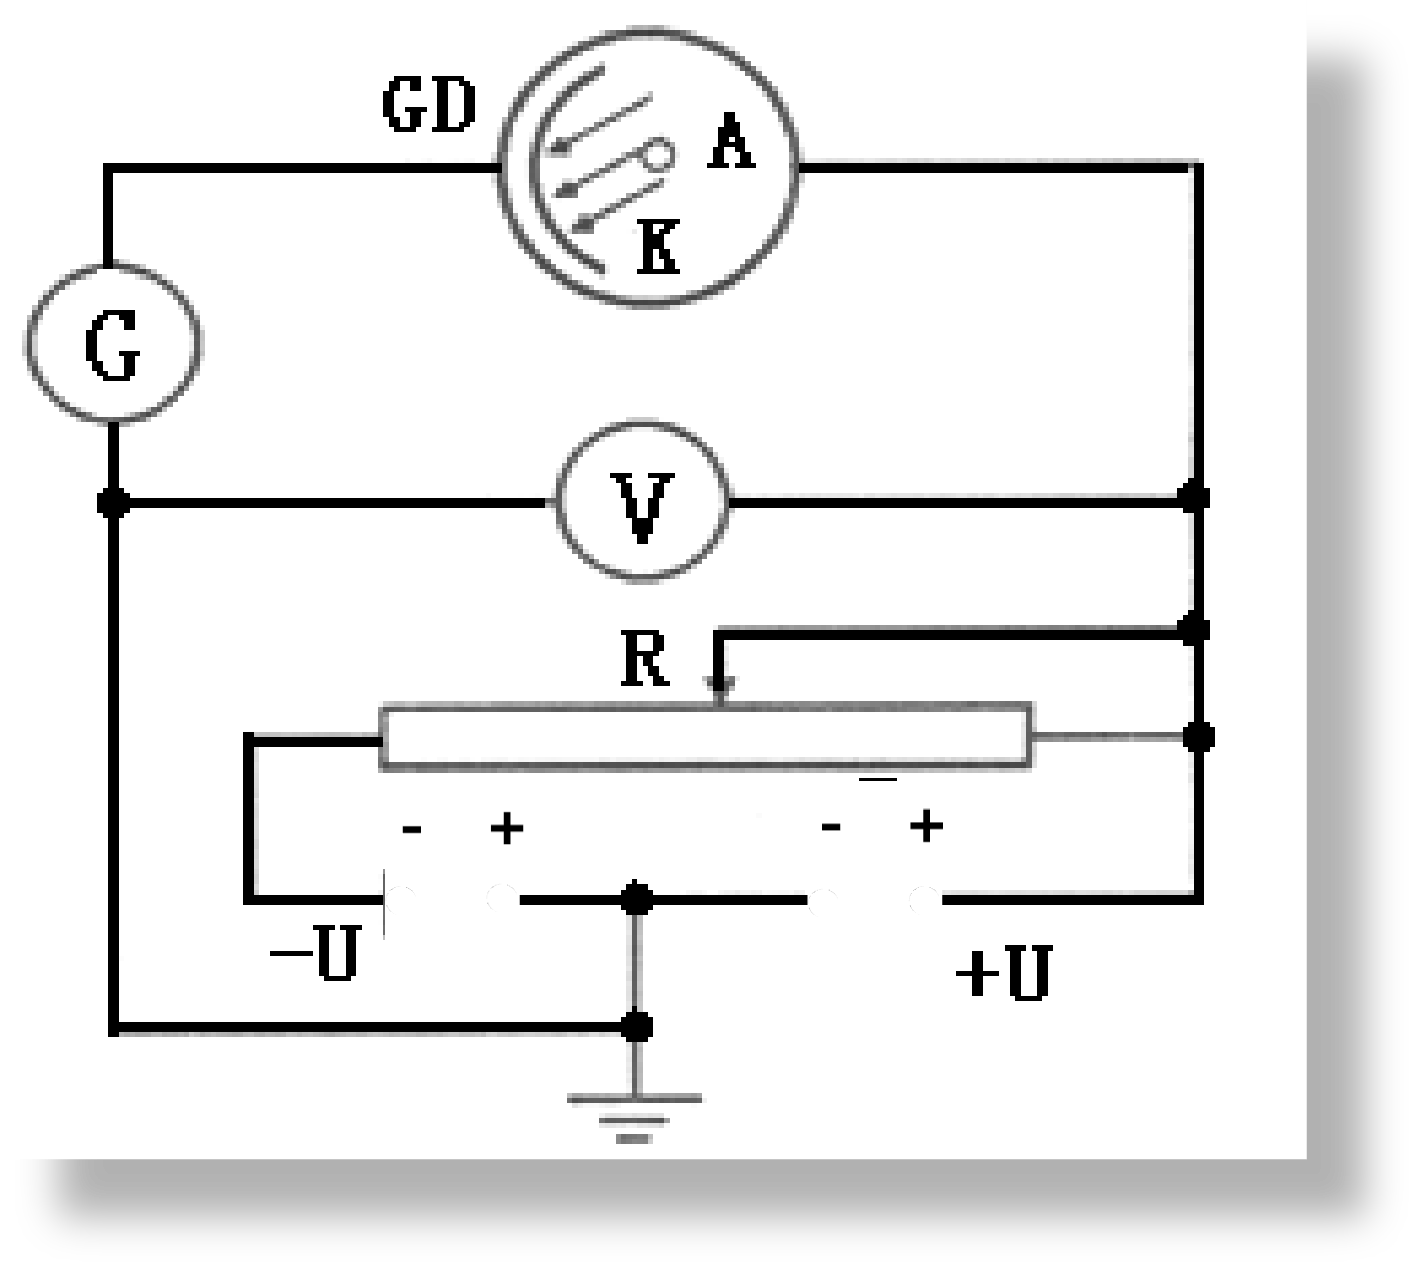
\includegraphics[width=0.35\textwidth]{figures/图1.png}
      \caption{光电效应实验示意图}
    \end{figure}

    图中，GD为光电管，K、A分别为阴极和阳极，G为微检流计，V为电压表，$\pm U$为电源，R为滑线变阻器。
    光照阴极使电子吸收光子能量后逸出，形成光电流；改变外加电压可测得伏安特性。

    光电效应具有以下规律：
    \begin{itemize}
      \item 光电子最大初动能随光频率线性变化，与光强无关；
      \item 光频率低于截止频率时，不产生光电子；
      \item 频率一定时，饱和光电流与光强成正比；
      \item 光电子发射具有瞬时性。
    \end{itemize}

    爱因斯坦光电效应方程为
    \[
    h\nu = \frac{1}{2}mv_{\max}^2 + W
    \]
    
    其中 $W$ 为阴极材料的逸出功。施加反向电压，使光电流恰好降为零时，其电压大小称为截止电压 $U_a$，满足 $eU_a=\frac{1}{2}mv_{\max}^2$。

    \begin{figure}[H]
      \centering
      \begin{minipage}{0.4\textwidth}
        \centering
        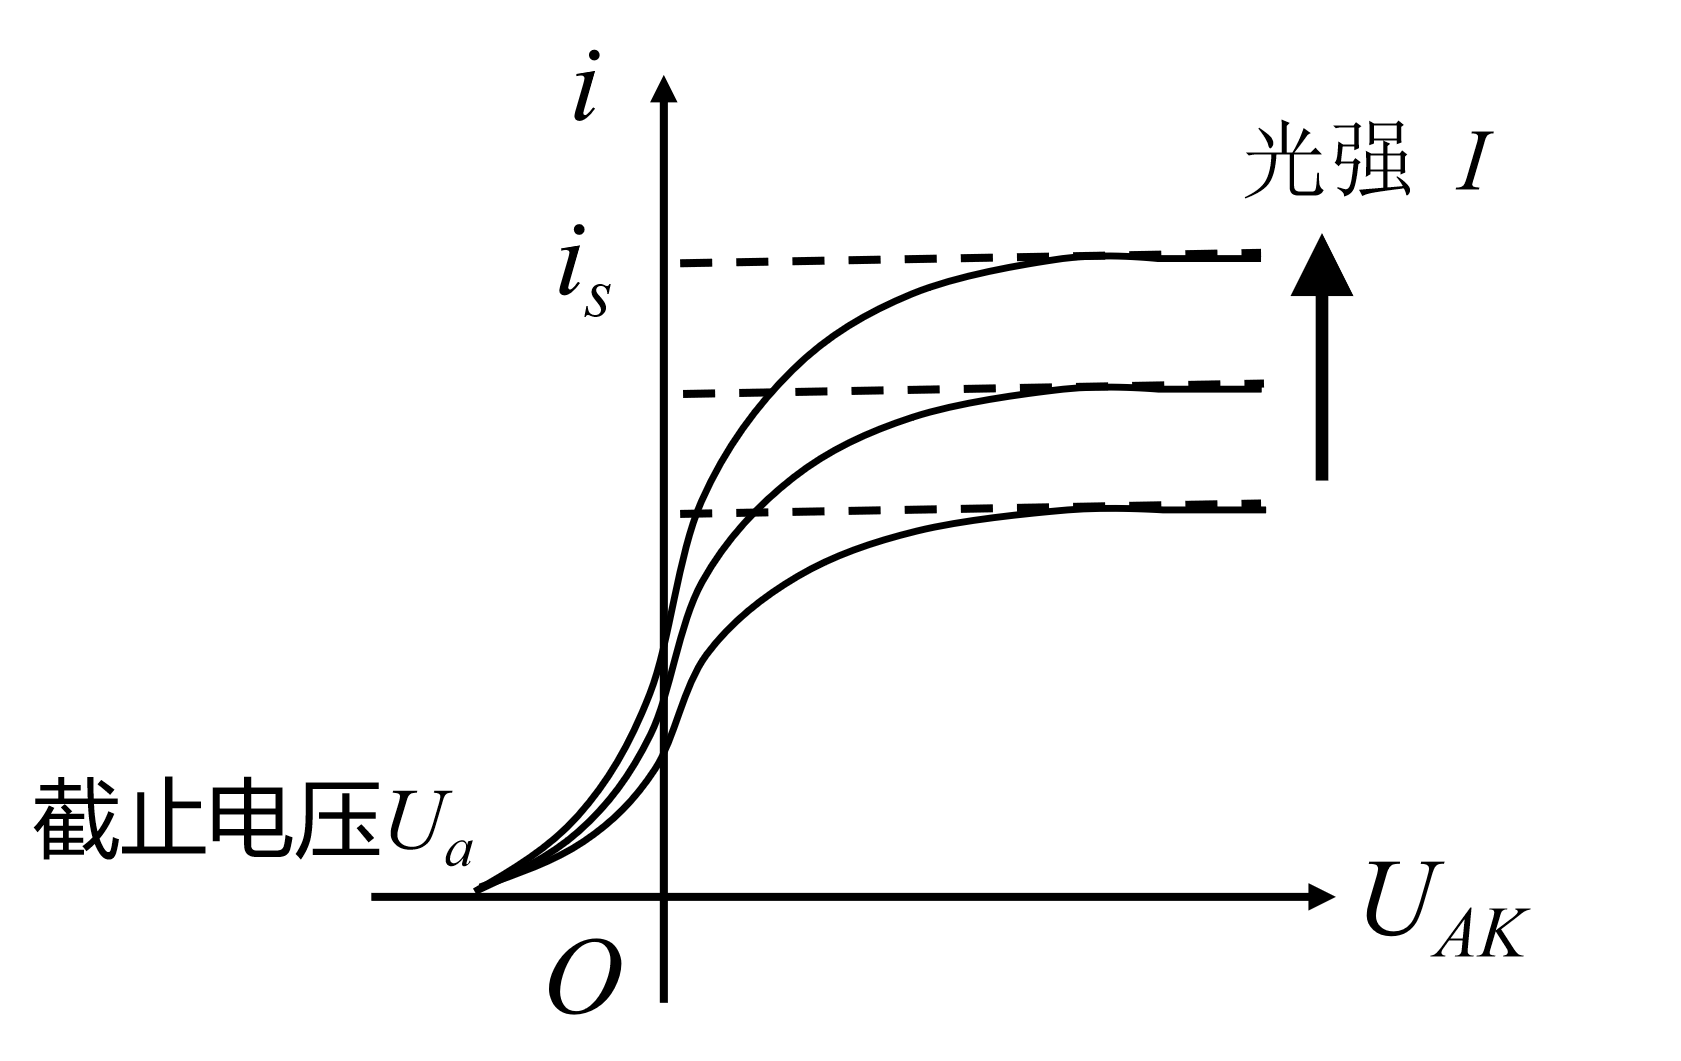
\includegraphics[width=\linewidth]{figures/图2.png}
        \caption{截止电压，饱和电流与光强}
      \end{minipage}
      \hfill
      \begin{minipage}{0.3\textwidth}
        \centering
        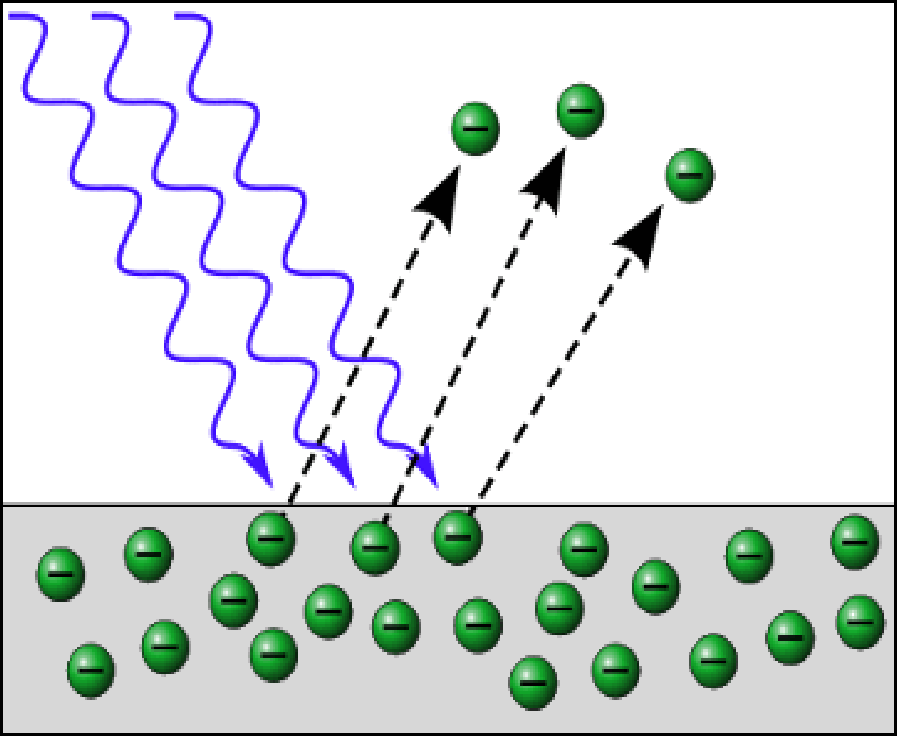
\includegraphics[width=\linewidth]{figures/图3.png}
        \caption{爱因斯坦光电效应方程}
      \end{minipage}
    \end{figure}

    \begin{wrapfigure}{r}{0.4\textwidth}
      \centering
      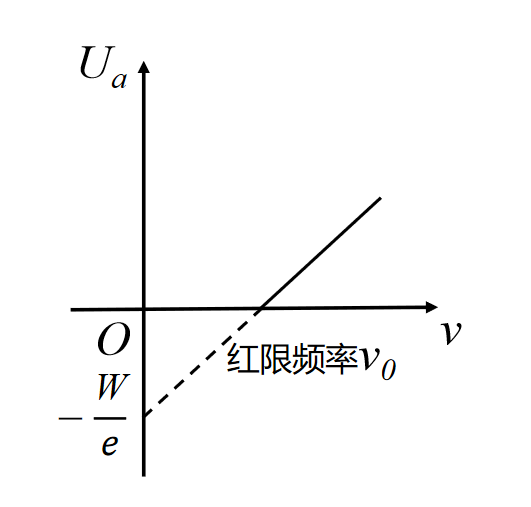
\includegraphics[width=\linewidth]{figures/图4.png}
      \caption{截止电压与频率的关系}
    \end{wrapfigure}

    由光电效应方程可得
    \[
    U_a = \frac{h}{e}\nu - \frac{W}{e},
    \qquad \nu_0 = \frac{W}{h}
    \]
    
    当 $\nu<\nu_0$ 时不发生光电效应；当 $\nu\geq\nu_0$ 时，截止电压与频率呈线性关系。
    测量不同频率下的截止电压并作线性拟合，由斜率 $k=h/e$ 求得 $h=ek$，由截距可求逸出功 $W$。

    \subsubsection{实验内容}
    \begin{enumerate}
      \item 使用不同滤光片，测量截止电压
      \item 使用不同滤光片，测量在单色光照射下的光电效应伏安特性曲线
      \item 在单色光照射下，探究光电管饱和光电流和光源距离的关系
      \item 在单色光照射下，探究光电管饱和光电流和光阑孔径大小的关系
    \end{enumerate} 

  \subsection{实验重点（3分）}
  \begin{enumerate}
    \item 理解光电效应方程和光量子概念
    \item 掌握光电效应实验方法并验证实验现象
    \item 测定普朗克常数
  \end{enumerate}

  \subsection{实验难点（2分）}
  \begin{enumerate}
    \item 准确判断光电流零点，测量各频率下的截止电压；
    \item 减小暗电流、接触电势及读数波动的影响；
    \item 对截止电压与频率作线性拟合，计算普朗克常量并分析误差。
  \end{enumerate}

\vspace*{\fill} % 使下面内容在页面底部显示
\noindent
\begin{minipage}{\textwidth}
  注意事项：

  \begingroup
    \setlength{\leftskip}{2em} % 1--4整体向右缩进两个汉字宽度
    1. 用PDF格式上传“实验报告”，文件名：学生姓名+学号+实验名称+周次。

    2. “实验报告”必须递交在“学在浙大”本课程内对应实验项目的“作业”模块内。

    3. “实验报告”成绩必须在“浙江大学物理实验教学中心网站”-“选课系统”内查询。

    4. 教学评价必须在“浙江大学物理实验教学中心网站”-“选课系统”内进行，学生必须进行教学评价，才能看到实验报告成绩，教学评价须在本次实验结束之后3天内进行。\par
  \endgroup

  \begin{center}
    {\CJKfontspec[AutoFakeBold=2.5]{SimSun}\bfseries 浙江大学物理实验教学中心制}
  \end{center}
\end{minipage}

\end{document}

